\documentclass[1p]{elsarticle_modified}
%\bibliographystyle{elsarticle-num}

%\usepackage[colorlinks]{hyperref}
%\usepackage{abbrmath_seonhwa} %\Abb, \Ascr, \Acal ,\Abf, \Afrak
\usepackage{amsfonts}
\usepackage{amssymb}
\usepackage{amsmath}
\usepackage{amsthm}
\usepackage{scalefnt}
\usepackage{amsbsy}
\usepackage{kotex}
\usepackage{caption}
\usepackage{subfig}
\usepackage{color}
\usepackage{graphicx}
\usepackage{xcolor} %% white, black, red, green, blue, cyan, magenta, yellow
\usepackage{float}
\usepackage{setspace}
\usepackage{hyperref}

\usepackage{tikz}
\usetikzlibrary{arrows}

\usepackage{multirow}
\usepackage{array} % fixed length table
\usepackage{hhline}

%%%%%%%%%%%%%%%%%%%%%
\makeatletter
\renewcommand*\env@matrix[1][\arraystretch]{%
	\edef\arraystretch{#1}%
	\hskip -\arraycolsep
	\let\@ifnextchar\new@ifnextchar
	\array{*\c@MaxMatrixCols c}}
\makeatother %https://tex.stackexchange.com/questions/14071/how-can-i-increase-the-line-spacing-in-a-matrix
%%%%%%%%%%%%%%%

\usepackage[normalem]{ulem}

\newcommand{\msout}[1]{\ifmmode\text{\sout{\ensuremath{#1}}}\else\sout{#1}\fi}
%SOURCE: \msout is \stkout macro in https://tex.stackexchange.com/questions/20609/strikeout-in-math-mode

\newcommand{\cancel}[1]{
	\ifmmode
	{\color{red}\msout{#1}}
	\else
	{\color{red}\sout{#1}}
	\fi
}

\newcommand{\add}[1]{
	{\color{blue}\uwave{#1}}
}

\newcommand{\replace}[2]{
	\ifmmode
	{\color{red}\msout{#1}}{\color{blue}\uwave{#2}}
	\else
	{\color{red}\sout{#1}}{\color{blue}\uwave{#2}}
	\fi
}

\newcommand{\Sol}{\mathcal{S}} %segment
\newcommand{\D}{D} %diagram
\newcommand{\A}{\mathcal{A}} %arc


%%%%%%%%%%%%%%%%%%%%%%%%%%%%%5 test

\def\sl{\operatorname{\textup{SL}}(2,\Cbb)}
\def\psl{\operatorname{\textup{PSL}}(2,\Cbb)}
\def\quan{\mkern 1mu \triangleright \mkern 1mu}

\theoremstyle{definition}
\newtheorem{thm}{Theorem}[section]
\newtheorem{prop}[thm]{Proposition}
\newtheorem{lem}[thm]{Lemma}
\newtheorem{ques}[thm]{Question}
\newtheorem{cor}[thm]{Corollary}
\newtheorem{defn}[thm]{Definition}
\newtheorem{exam}[thm]{Example}
\newtheorem{rmk}[thm]{Remark}
\newtheorem{alg}[thm]{Algorithm}

\newcommand{\I}{\sqrt{-1}}
\begin{document}

%\begin{frontmatter}
%
%\title{Boundary parabolic representations of knots up to 8 crossings}
%
%%% Group authors per affiliation:
%\author{Yunhi Cho} 
%\address{Department of Mathematics, University of Seoul, Seoul, Korea}
%\ead{yhcho@uos.ac.kr}
%
%
%\author{Seonhwa Kim} %\fnref{s_kim}}
%\address{Center for Geometry and Physics, Institute for Basic Science, Pohang, 37673, Korea}
%\ead{ryeona17@ibs.re.kr}
%
%\author{Hyuk Kim}
%\address{Department of Mathematical Sciences, Seoul National University, Seoul 08826, Korea}
%\ead{hyukkim@snu.ac.kr}
%
%\author{Seokbeom Yoon}
%\address{Department of Mathematical Sciences, Seoul National University, Seoul, 08826,  Korea}
%\ead{sbyoon15@snu.ac.kr}
%
%\begin{abstract}
%We find all boundary parabolic representation of knots up to 8 crossings.
%
%\end{abstract}
%\begin{keyword}
%    \MSC[2010] 57M25 
%\end{keyword}
%
%\end{frontmatter}

%\linenumbers
%\tableofcontents
%
\newcommand\colored[1]{\textcolor{white}{\rule[-0.35ex]{0.8em}{1.4ex}}\kern-0.8em\color{red} #1}%
%\newcommand\colored[1]{\textcolor{white}{ #1}\kern-2.17ex	\textcolor{white}{ #1}\kern-1.81ex	\textcolor{white}{ #1}\kern-2.15ex\color{red}#1	}

{\Large $\underline{11n_{132}~(K11n_{132})}$}

\setlength{\tabcolsep}{10pt}
\renewcommand{\arraystretch}{1.6}
\vspace{1cm}\begin{tabular}{m{100pt}>{\centering\arraybackslash}m{274pt}}
\multirow{5}{120pt}{
	\centering
	\includegraphics[width=112pt]{../../../GIT/diagram.site/Diagrams/png/748_11n_132.png}\\
\ \ \ A knot diagram\footnotemark}&
\allowdisplaybreaks
\textbf{Linearized knot diagam} \\
\cline{2-2}
 &
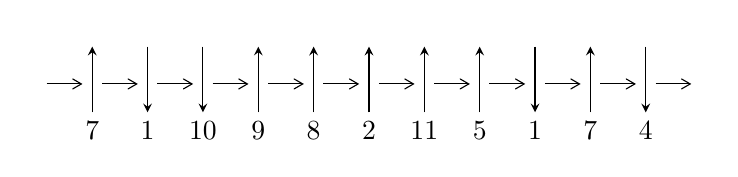
\begin{tikzpicture}[x=20pt, y=17pt]
	% nodes
	\node (C0) at (0, 0) {};
	\node (C1) at (1, 0) {};
	\node (C1U) at (1, +1) {};
	\node (C1D) at (1, -1) {7};

	\node (C2) at (2, 0) {};
	\node (C2U) at (2, +1) {};
	\node (C2D) at (2, -1) {1};

	\node (C3) at (3, 0) {};
	\node (C3U) at (3, +1) {};
	\node (C3D) at (3, -1) {10};

	\node (C4) at (4, 0) {};
	\node (C4U) at (4, +1) {};
	\node (C4D) at (4, -1) {9};

	\node (C5) at (5, 0) {};
	\node (C5U) at (5, +1) {};
	\node (C5D) at (5, -1) {8};

	\node (C6) at (6, 0) {};
	\node (C6U) at (6, +1) {};
	\node (C6D) at (6, -1) {2};

	\node (C7) at (7, 0) {};
	\node (C7U) at (7, +1) {};
	\node (C7D) at (7, -1) {11};

	\node (C8) at (8, 0) {};
	\node (C8U) at (8, +1) {};
	\node (C8D) at (8, -1) {5};

	\node (C9) at (9, 0) {};
	\node (C9U) at (9, +1) {};
	\node (C9D) at (9, -1) {1};

	\node (C10) at (10, 0) {};
	\node (C10U) at (10, +1) {};
	\node (C10D) at (10, -1) {7};

	\node (C11) at (11, 0) {};
	\node (C11U) at (11, +1) {};
	\node (C11D) at (11, -1) {4};
	\node (C12) at (12, 0) {};

	% arrows
	\draw[->,>={angle 60}]
	(C0) edge (C1) (C1) edge (C2) (C2) edge (C3) (C3) edge (C4) (C4) edge (C5) (C5) edge (C6) (C6) edge (C7) (C7) edge (C8) (C8) edge (C9) (C9) edge (C10) (C10) edge (C11) (C11) edge (C12) ;	\draw[->,>=stealth]
	(C1D) edge (C1U) (C2U) edge (C2D) (C3U) edge (C3D) (C4D) edge (C4U) (C5D) edge (C5U) (C6D) edge (C6U) (C7D) edge (C7U) (C8D) edge (C8U) (C9U) edge (C9D) (C10D) edge (C10U) (C11U) edge (C11D) ;
	\end{tikzpicture} \\
\hhline{~~} \\& 
\textbf{Solving Sequence} \\ \cline{2-2} 
 &
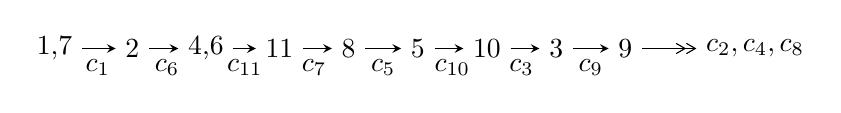
\begin{tikzpicture}[x=25pt, y=7pt]
	% node
	\node (A0) at (-1/8, 0) {1,7};
	\node (A1) at (1, 0) {2};
	\node (A2) at (33/16, 0) {4,6};
	\node (A3) at (25/8, 0) {11};
	\node (A4) at (33/8, 0) {8};
	\node (A5) at (41/8, 0) {5};
	\node (A6) at (49/8, 0) {10};
	\node (A7) at (57/8, 0) {3};
	\node (A8) at (65/8, 0) {9};
	\node (C1) at (1/2, -1) {$c_{1}$};
	\node (C2) at (3/2, -1) {$c_{6}$};
	\node (C3) at (21/8, -1) {$c_{11}$};
	\node (C4) at (29/8, -1) {$c_{7}$};
	\node (C5) at (37/8, -1) {$c_{5}$};
	\node (C6) at (45/8, -1) {$c_{10}$};
	\node (C7) at (53/8, -1) {$c_{3}$};
	\node (C8) at (61/8, -1) {$c_{9}$};
	\node (A9) at (10, 0) {$c_{2},c_{4},c_{8}$};

	% edge
	\draw[->,>=stealth]	
	(A0) edge (A1) (A1) edge (A2) (A2) edge (A3) (A3) edge (A4) (A4) edge (A5) (A5) edge (A6) (A6) edge (A7) (A7) edge (A8) ;
	\draw[->>,>={angle 60}]	
	(A8) edge (A9);
\end{tikzpicture} \\ 

\end{tabular} \\

\footnotetext{
The image of knot diagram is generated by the software ``\textbf{Draw programme}" developed by Andrew Bartholomew(\url{http://www.layer8.co.uk/maths/draw/index.htm\#Running-draw}), where we modified some parts for our purpose(\url{https://github.com/CATsTAILs/LinksPainter}).
}\phantom \\ \newline 
\centering \textbf{Ideals for irreducible components\footnotemark of $X_{\text{par}}$} 
 
\begin{align*}
I^u_{1}&=\langle 
-7.33308\times10^{15} u^{20}-1.72888\times10^{17} u^{19}+\cdots+1.09599\times10^{19} b-8.78124\times10^{18},\\
\phantom{I^u_{1}}&\phantom{= \langle  }-2.80505\times10^{18} u^{20}+4.20368\times10^{18} u^{19}+\cdots+7.67190\times10^{19} a-6.10889\times10^{19},\\
\phantom{I^u_{1}}&\phantom{= \langle  }u^{21}- u^{20}+\cdots-18 u+28\rangle \\
I^u_{2}&=\langle 
u^8+3 u^6+u^5+2 u^4+u^3+u^2+b+u-1,\;- u^2+a-2,\;u^9+4 u^7+u^6+5 u^5+2 u^4+3 u^3+2 u^2+1\rangle \\
\\
\end{align*}
\raggedright * 2 irreducible components of $\dim_{\mathbb{C}}=0$, with total 30 representations.\\
\footnotetext{All coefficients of polynomials are rational numbers. But the coefficients are sometimes approximated in decimal forms when there is not enough margin.}
\newpage
\renewcommand{\arraystretch}{1}
\centering \section*{I. $I^u_{1}= \langle -7.33\times10^{15} u^{20}-1.73\times10^{17} u^{19}+\cdots+1.10\times10^{19} b-8.78\times10^{18},\;-2.81\times10^{18} u^{20}+4.20\times10^{18} u^{19}+\cdots+7.67\times10^{19} a-6.11\times10^{19},\;u^{21}- u^{20}+\cdots-18 u+28 \rangle$}
\flushleft \textbf{(i) Arc colorings}\\
\begin{tabular}{m{7pt} m{180pt} m{7pt} m{180pt} }
\flushright $a_{1}=$&$\begin{pmatrix}1\\0\end{pmatrix}$ \\
\flushright $a_{7}=$&$\begin{pmatrix}0\\u\end{pmatrix}$ \\
\flushright $a_{2}=$&$\begin{pmatrix}1\\- u^2\end{pmatrix}$ \\
\flushright $a_{4}=$&$\begin{pmatrix}0.0365627 u^{20}-0.0547932 u^{19}+\cdots+1.60738 u+0.796268\\0.000669086 u^{20}+0.0157746 u^{19}+\cdots-0.933535 u+0.801219\end{pmatrix}$ \\
\flushright $a_{6}=$&$\begin{pmatrix}- u\\u^3+u\end{pmatrix}$ \\
\flushright $a_{11}=$&$\begin{pmatrix}-0.0196295 u^{20}-0.0100507 u^{19}+\cdots+1.18048 u+0.217188\\0.00797850 u^{20}-0.0158077 u^{19}+\cdots+0.180611 u-0.795772\end{pmatrix}$ \\
\flushright $a_{8}=$&$\begin{pmatrix}-0.0142692 u^{20}+0.0411108 u^{19}+\cdots-0.773349 u+1.95583\\-0.00351504 u^{20}+0.0137854 u^{19}+\cdots-0.476341 u+0.0864955\end{pmatrix}$ \\
\flushright $a_{5}=$&$\begin{pmatrix}0.0138798 u^{20}-0.0293691 u^{19}+\cdots+1.58093 u+0.793197\\0.00952514 u^{20}-0.0122960 u^{19}+\cdots+0.486832 u+0.362072\end{pmatrix}$ \\
\flushright $a_{10}=$&$\begin{pmatrix}-0.0196295 u^{20}-0.0100507 u^{19}+\cdots+1.18048 u+0.217188\\0.0175759 u^{20}-0.0166603 u^{19}+\cdots+0.195992 u+0.0352752\end{pmatrix}$ \\
\flushright $a_{3}=$&$\begin{pmatrix}u^2+1\\- u^2\end{pmatrix}$ \\
\flushright $a_{9}=$&$\begin{pmatrix}-0.00205357 u^{20}-0.0267111 u^{19}+\cdots+1.37648 u+0.252463\\0.0175759 u^{20}-0.0166603 u^{19}+\cdots+0.195992 u+0.0352752\end{pmatrix}$\\ \flushright $a_{9}=$&$\begin{pmatrix}-0.00205357 u^{20}-0.0267111 u^{19}+\cdots+1.37648 u+0.252463\\0.0175759 u^{20}-0.0166603 u^{19}+\cdots+0.195992 u+0.0352752\end{pmatrix}$\\&\end{tabular}
\flushleft \textbf{(ii) Obstruction class $= -1$}\\~\\
\flushleft \textbf{(iii) Cusp Shapes $= \frac{445709904941671169}{2739962993558394514} u^{20}-\frac{891361635722125989}{5479925987116789028} u^{19}+\cdots+\frac{14080564157258258655}{2739962993558394514} u+\frac{2949485749258559055}{1369981496779197257}$}\\~\\
\newpage\renewcommand{\arraystretch}{1}
\flushleft \textbf{(iv) u-Polynomials at the component}\newline \\
\begin{tabular}{m{50pt}|m{274pt}}
Crossings & \hspace{64pt}u-Polynomials at each crossing \\
\hline $$\begin{aligned}c_{1},c_{6}\end{aligned}$$&$\begin{aligned}
&u^{21}+u^{20}+\cdots-18 u-28
\end{aligned}$\\
\hline $$\begin{aligned}c_{2}\end{aligned}$$&$\begin{aligned}
&u^{21}+33 u^{20}+\cdots-1972 u-784
\end{aligned}$\\
\hline $$\begin{aligned}c_{3}\end{aligned}$$&$\begin{aligned}
&u^{21}-24 u^{19}+\cdots+1851 u-281
\end{aligned}$\\
\hline $$\begin{aligned}c_{4},c_{5},c_{8}\end{aligned}$$&$\begin{aligned}
&u^{21}+2 u^{20}+\cdots-12 u-11
\end{aligned}$\\
\hline $$\begin{aligned}c_{7},c_{10}\end{aligned}$$&$\begin{aligned}
&u^{21}-3 u^{20}+\cdots-10 u-47
\end{aligned}$\\
\hline $$\begin{aligned}c_{9}\end{aligned}$$&$\begin{aligned}
&u^{21}-17 u^{19}+\cdots+73 u-13
\end{aligned}$\\
\hline $$\begin{aligned}c_{11}\end{aligned}$$&$\begin{aligned}
&u^{21}-4 u^{20}+\cdots+19 u-1
\end{aligned}$\\
\hline
\end{tabular}\\~\\
\newpage\renewcommand{\arraystretch}{1}
\flushleft \textbf{(v) Riley Polynomials at the component}\newline \\
\begin{tabular}{m{50pt}|m{274pt}}
Crossings & \hspace{64pt}Riley Polynomials at each crossing \\
\hline $$\begin{aligned}c_{1},c_{6}\end{aligned}$$&$\begin{aligned}
&y^{21}+33 y^{20}+\cdots-1972 y-784
\end{aligned}$\\
\hline $$\begin{aligned}c_{2}\end{aligned}$$&$\begin{aligned}
&y^{21}-87 y^{20}+\cdots+22145008 y-614656
\end{aligned}$\\
\hline $$\begin{aligned}c_{3}\end{aligned}$$&$\begin{aligned}
&y^{21}-48 y^{20}+\cdots+982063 y-78961
\end{aligned}$\\
\hline $$\begin{aligned}c_{4},c_{5},c_{8}\end{aligned}$$&$\begin{aligned}
&y^{21}+26 y^{20}+\cdots-846 y-121
\end{aligned}$\\
\hline $$\begin{aligned}c_{7},c_{10}\end{aligned}$$&$\begin{aligned}
&y^{21}+7 y^{20}+\cdots-7232 y-2209
\end{aligned}$\\
\hline $$\begin{aligned}c_{9}\end{aligned}$$&$\begin{aligned}
&y^{21}-34 y^{20}+\cdots+2495 y-169
\end{aligned}$\\
\hline $$\begin{aligned}c_{11}\end{aligned}$$&$\begin{aligned}
&y^{21}-4 y^{20}+\cdots+319 y-1
\end{aligned}$\\
\hline
\end{tabular}\\~\\
\newpage\flushleft \textbf{(vi) Complex Volumes and Cusp Shapes}
$$\begin{array}{c|c|c}  
\text{Solutions to }I^u_{1}& \I (\text{vol} + \sqrt{-1}CS) & \text{Cusp shape}\\
 \hline 
\begin{aligned}
u &= -0.667126 + 0.763695 I \\
a &= \phantom{-}0.82594 - 1.23941 I \\
b &= \phantom{-}0.258218 + 1.151380 I\end{aligned}
 & \phantom{-}1.34010 - 2.53227 I & \phantom{-}0.85890 + 6.43019 I \\ \hline\begin{aligned}
u &= -0.667126 - 0.763695 I \\
a &= \phantom{-}0.82594 + 1.23941 I \\
b &= \phantom{-}0.258218 - 1.151380 I\end{aligned}
 & \phantom{-}1.34010 + 2.53227 I & \phantom{-}0.85890 - 6.43019 I \\ \hline\begin{aligned}
u &= -0.354561 + 1.008430 I \\
a &= -0.227436 + 0.200357 I \\
b &= \phantom{-}0.917813 - 0.821950 I\end{aligned}
 & -7.02572 + 3.49738 I & -2.24629 - 2.87148 I \\ \hline\begin{aligned}
u &= -0.354561 - 1.008430 I \\
a &= -0.227436 - 0.200357 I \\
b &= \phantom{-}0.917813 + 0.821950 I\end{aligned}
 & -7.02572 - 3.49738 I & -2.24629 + 2.87148 I \\ \hline\begin{aligned}
u &= -0.135425 + 0.749831 I \\
a &= \phantom{-}2.26639 + 0.24841 I \\
b &= \phantom{-}0.299503 - 0.694156 I\end{aligned}
 & \phantom{-}1.72913 + 0.18094 I & \phantom{-}3.57258 - 0.16926 I \\ \hline\begin{aligned}
u &= -0.135425 - 0.749831 I \\
a &= \phantom{-}2.26639 - 0.24841 I \\
b &= \phantom{-}0.299503 + 0.694156 I\end{aligned}
 & \phantom{-}1.72913 - 0.18094 I & \phantom{-}3.57258 + 0.16926 I \\ \hline\begin{aligned}
u &= \phantom{-}0.137433 + 0.625721 I \\
a &= \phantom{-}0.041014 - 0.214438 I \\
b &= \phantom{-}0.721689 + 0.405487 I\end{aligned}
 & -1.28019 - 1.09527 I & -2.70112 + 3.21254 I \\ \hline\begin{aligned}
u &= \phantom{-}0.137433 - 0.625721 I \\
a &= \phantom{-}0.041014 + 0.214438 I \\
b &= \phantom{-}0.721689 - 0.405487 I\end{aligned}
 & -1.28019 + 1.09527 I & -2.70112 - 3.21254 I \\ \hline\begin{aligned}
u &= \phantom{-}0.576539 + 0.104726 I \\
a &= \phantom{-}0.14734 - 1.76070 I \\
b &= -0.906943 - 0.072981 I\end{aligned}
 & -4.46536 - 3.00711 I & \phantom{-}1.90224 + 0.80232 I \\ \hline\begin{aligned}
u &= \phantom{-}0.576539 - 0.104726 I \\
a &= \phantom{-}0.14734 + 1.76070 I \\
b &= -0.906943 + 0.072981 I\end{aligned}
 & -4.46536 + 3.00711 I & \phantom{-}1.90224 - 0.80232 I\\
 \hline 
 \end{array}$$\newpage$$\begin{array}{c|c|c}  
\text{Solutions to }I^u_{1}& \I (\text{vol} + \sqrt{-1}CS) & \text{Cusp shape}\\
 \hline 
\begin{aligned}
u &= -0.534365\phantom{ +0.000000I} \\
a &= \phantom{-}2.09662\phantom{ +0.000000I} \\
b &= -0.0562424\phantom{ +0.000000I}\end{aligned}
 & \phantom{-}1.11788\phantom{ +0.000000I} & \phantom{-}11.2410\phantom{ +0.000000I} \\ \hline\begin{aligned}
u &= \phantom{-}0.07520 + 1.61647 I \\
a &= -0.453620 - 0.070826 I \\
b &= -0.793621 - 0.491574 I\end{aligned}
 & -8.87305 + 0.26805 I & -1.47803 + 0.75243 I \\ \hline\begin{aligned}
u &= \phantom{-}0.07520 - 1.61647 I \\
a &= -0.453620 + 0.070826 I \\
b &= -0.793621 + 0.491574 I\end{aligned}
 & -8.87305 - 0.26805 I & -1.47803 - 0.75243 I \\ \hline\begin{aligned}
u &= \phantom{-}1.10769 + 1.23434 I \\
a &= \phantom{-}0.723626 + 0.961597 I \\
b &= \phantom{-}1.194160 - 0.750185 I\end{aligned}
 & -7.93629 + 2.97451 I & -2.24011 - 2.11283 I \\ \hline\begin{aligned}
u &= \phantom{-}1.10769 - 1.23434 I \\
a &= \phantom{-}0.723626 - 0.961597 I \\
b &= \phantom{-}1.194160 + 0.750185 I\end{aligned}
 & -7.93629 - 2.97451 I & -2.24011 + 2.11283 I \\ \hline\begin{aligned}
u &= -0.31257 + 1.99292 I \\
a &= -0.345671 + 0.172538 I \\
b &= -1.21980 + 1.39213 I\end{aligned}
 & -17.7841 - 0.7836 I & -1.50922 + 0.14627 I \\ \hline\begin{aligned}
u &= -0.31257 - 1.99292 I \\
a &= -0.345671 - 0.172538 I \\
b &= -1.21980 - 1.39213 I\end{aligned}
 & -17.7841 + 0.7836 I & -1.50922 - 0.14627 I \\ \hline\begin{aligned}
u &= \phantom{-}0.42977 + 2.01390 I \\
a &= -0.984072 - 0.475371 I \\
b &= -1.34381 + 1.14589 I\end{aligned}
 & -18.4994 + 10.2668 I & -1.32790 - 4.15834 I \\ \hline\begin{aligned}
u &= \phantom{-}0.42977 - 2.01390 I \\
a &= -0.984072 + 0.475371 I \\
b &= -1.34381 - 1.14589 I\end{aligned}
 & -18.4994 - 10.2668 I & -1.32790 + 4.15834 I \\ \hline\begin{aligned}
u &= -0.08976 + 2.09219 I \\
a &= -1.363250 + 0.356504 I \\
b &= -1.099090 - 0.439233 I\end{aligned}
 & -10.14110 - 4.18838 I & -1.95156 + 4.03302 I\\
 \hline 
 \end{array}$$\newpage$$\begin{array}{c|c|c}  
\text{Solutions to }I^u_{1}& \I (\text{vol} + \sqrt{-1}CS) & \text{Cusp shape}\\
 \hline 
\begin{aligned}
u &= -0.08976 - 2.09219 I \\
a &= -1.363250 - 0.356504 I \\
b &= -1.099090 + 0.439233 I\end{aligned}
 & -10.14110 + 4.18838 I & -1.95156 - 4.03302 I\\
 \hline 
 \end{array}$$\newpage\newpage\renewcommand{\arraystretch}{1}
\centering \section*{II. $I^u_{2}= \langle u^8+3 u^6+u^5+2 u^4+u^3+u^2+b+u-1,\;- u^2+a-2,\;u^9+4 u^7+u^6+5 u^5+2 u^4+3 u^3+2 u^2+1 \rangle$}
\flushleft \textbf{(i) Arc colorings}\\
\begin{tabular}{m{7pt} m{180pt} m{7pt} m{180pt} }
\flushright $a_{1}=$&$\begin{pmatrix}1\\0\end{pmatrix}$ \\
\flushright $a_{7}=$&$\begin{pmatrix}0\\u\end{pmatrix}$ \\
\flushright $a_{2}=$&$\begin{pmatrix}1\\- u^2\end{pmatrix}$ \\
\flushright $a_{4}=$&$\begin{pmatrix}u^2+2\\- u^8-3 u^6- u^5-2 u^4- u^3- u^2- u+1\end{pmatrix}$ \\
\flushright $a_{6}=$&$\begin{pmatrix}- u\\u^3+u\end{pmatrix}$ \\
\flushright $a_{11}=$&$\begin{pmatrix}u^8+3 u^6+u^5+2 u^4+u^3+u^2+u-1\\2 u^8+u^7+7 u^6+5 u^5+7 u^4+5 u^3+3 u^2+3 u\end{pmatrix}$ \\
\flushright $a_{8}=$&$\begin{pmatrix}- u^8+u^7-3 u^6+3 u^5- u^4+3 u^3+u^2+2\\-2 u^8- u^7-7 u^6-4 u^5-7 u^4-2 u^3-2 u^2- u+1\end{pmatrix}$ \\
\flushright $a_{5}=$&$\begin{pmatrix}u^8+3 u^6+u^4-2 u^3-2 u^2-2 u-1\\- u^8-3 u^6- u^5-2 u^4- u^3-2 u^2-2 u\end{pmatrix}$ \\
\flushright $a_{10}=$&$\begin{pmatrix}u^8+3 u^6+u^5+2 u^4+u^3+u^2+u-1\\u^8+u^7+4 u^6+4 u^5+5 u^4+4 u^3+2 u^2+2 u\end{pmatrix}$ \\
\flushright $a_{3}=$&$\begin{pmatrix}u^2+1\\- u^2\end{pmatrix}$ \\
\flushright $a_{9}=$&$\begin{pmatrix}2 u^8+u^7+7 u^6+5 u^5+7 u^4+5 u^3+3 u^2+3 u-1\\u^8+u^7+4 u^6+4 u^5+5 u^4+4 u^3+2 u^2+2 u\end{pmatrix}$\\ \flushright $a_{9}=$&$\begin{pmatrix}2 u^8+u^7+7 u^6+5 u^5+7 u^4+5 u^3+3 u^2+3 u-1\\u^8+u^7+4 u^6+4 u^5+5 u^4+4 u^3+2 u^2+2 u\end{pmatrix}$\\&\end{tabular}
\flushleft \textbf{(ii) Obstruction class $= 1$}\\~\\
\flushleft \textbf{(iii) Cusp Shapes $= -2 u^8-3 u^7-8 u^6-12 u^5-15 u^4-12 u^3-14 u^2-7 u-4$}\\~\\
\newpage\renewcommand{\arraystretch}{1}
\flushleft \textbf{(iv) u-Polynomials at the component}\newline \\
\begin{tabular}{m{50pt}|m{274pt}}
Crossings & \hspace{64pt}u-Polynomials at each crossing \\
\hline $$\begin{aligned}c_{1}\end{aligned}$$&$\begin{aligned}
&u^9+4 u^7+u^6+5 u^5+2 u^4+3 u^3+2 u^2+1
\end{aligned}$\\
\hline $$\begin{aligned}c_{2}\end{aligned}$$&$\begin{aligned}
&u^9+8 u^8+26 u^7+45 u^6+45 u^5+22 u^4- u^3-8 u^2-4 u-1
\end{aligned}$\\
\hline $$\begin{aligned}c_{3}\end{aligned}$$&$\begin{aligned}
&u^9+u^8-2 u^7-3 u^6- u^5+4 u^4+7 u^3+6 u^2+3 u+1
\end{aligned}$\\
\hline $$\begin{aligned}c_{4},c_{5}\end{aligned}$$&$\begin{aligned}
&u^9+u^8+5 u^7+5 u^6+9 u^5+10 u^4+7 u^3+8 u^2+2 u+1
\end{aligned}$\\
\hline $$\begin{aligned}c_{6}\end{aligned}$$&$\begin{aligned}
&u^9+4 u^7- u^6+5 u^5-2 u^4+3 u^3-2 u^2-1
\end{aligned}$\\
\hline $$\begin{aligned}c_{7}\end{aligned}$$&$\begin{aligned}
&u^9-2 u^8- u^7+4 u^6-3 u^5+4 u^3-3 u^2+1
\end{aligned}$\\
\hline $$\begin{aligned}c_{8}\end{aligned}$$&$\begin{aligned}
&u^9- u^8+5 u^7-5 u^6+9 u^5-10 u^4+7 u^3-8 u^2+2 u-1
\end{aligned}$\\
\hline $$\begin{aligned}c_{9}\end{aligned}$$&$\begin{aligned}
&u^9-3 u^8- u^7+9 u^6-2 u^5-10 u^4+7 u^3+2 u^2- u-1
\end{aligned}$\\
\hline $$\begin{aligned}c_{10}\end{aligned}$$&$\begin{aligned}
&u^9+2 u^8- u^7-4 u^6-3 u^5+4 u^3+3 u^2-1
\end{aligned}$\\
\hline $$\begin{aligned}c_{11}\end{aligned}$$&$\begin{aligned}
&u^9-3 u^8+6 u^7-7 u^6+4 u^5+u^4-3 u^3+2 u^2+u-1
\end{aligned}$\\
\hline
\end{tabular}\\~\\
\newpage\renewcommand{\arraystretch}{1}
\flushleft \textbf{(v) Riley Polynomials at the component}\newline \\
\begin{tabular}{m{50pt}|m{274pt}}
Crossings & \hspace{64pt}Riley Polynomials at each crossing \\
\hline $$\begin{aligned}c_{1},c_{6}\end{aligned}$$&$\begin{aligned}
&y^9+8 y^8+26 y^7+45 y^6+45 y^5+22 y^4- y^3-8 y^2-4 y-1
\end{aligned}$\\
\hline $$\begin{aligned}c_{2}\end{aligned}$$&$\begin{aligned}
&y^9-12 y^8+46 y^7-39 y^6+113 y^5-46 y^4+83 y^3-12 y^2-1
\end{aligned}$\\
\hline $$\begin{aligned}c_{3}\end{aligned}$$&$\begin{aligned}
&y^9-5 y^8+8 y^7+y^6-9 y^5-8 y^4+y^3-2 y^2-3 y-1
\end{aligned}$\\
\hline $$\begin{aligned}c_{4},c_{5},c_{8}\end{aligned}$$&$\begin{aligned}
&y^9+9 y^8+33 y^7+59 y^6+39 y^5-36 y^4-85 y^3-56 y^2-12 y-1
\end{aligned}$\\
\hline $$\begin{aligned}c_{7},c_{10}\end{aligned}$$&$\begin{aligned}
&y^9-6 y^8+11 y^7-2 y^6-11 y^5+4 y^4+8 y^3-9 y^2+6 y-1
\end{aligned}$\\
\hline $$\begin{aligned}c_{9}\end{aligned}$$&$\begin{aligned}
&y^9-11 y^8+51 y^7-123 y^6+180 y^5-168 y^4+111 y^3-38 y^2+5 y-1
\end{aligned}$\\
\hline $$\begin{aligned}c_{11}\end{aligned}$$&$\begin{aligned}
&y^9+3 y^8+2 y^7- y^6+8 y^5+9 y^4- y^3-8 y^2+5 y-1
\end{aligned}$\\
\hline
\end{tabular}\\~\\
\newpage\flushleft \textbf{(vi) Complex Volumes and Cusp Shapes}
$$\begin{array}{c|c|c}  
\text{Solutions to }I^u_{2}& \I (\text{vol} + \sqrt{-1}CS) & \text{Cusp shape}\\
 \hline 
\begin{aligned}
u &= \phantom{-}0.338665 + 0.974837 I \\
a &= \phantom{-}1.164390 + 0.660286 I \\
b &= \phantom{-}0.35504 - 1.42610 I\end{aligned}
 & -1.24626 + 1.32727 I & -0.553077 - 1.214568 I \\ \hline\begin{aligned}
u &= \phantom{-}0.338665 - 0.974837 I \\
a &= \phantom{-}1.164390 - 0.660286 I \\
b &= \phantom{-}0.35504 + 1.42610 I\end{aligned}
 & -1.24626 - 1.32727 I & -0.553077 + 1.214568 I \\ \hline\begin{aligned}
u &= -0.447524 + 0.951550 I \\
a &= \phantom{-}1.29483 - 0.85168 I \\
b &= \phantom{-}0.362962 + 1.048500 I\end{aligned}
 & \phantom{-}1.95197 - 1.71727 I & \phantom{-}4.44186 + 1.84082 I \\ \hline\begin{aligned}
u &= -0.447524 - 0.951550 I \\
a &= \phantom{-}1.29483 + 0.85168 I \\
b &= \phantom{-}0.362962 - 1.048500 I\end{aligned}
 & \phantom{-}1.95197 + 1.71727 I & \phantom{-}4.44186 - 1.84082 I \\ \hline\begin{aligned}
u &= -0.738179\phantom{ +0.000000I} \\
a &= \phantom{-}2.54491\phantom{ +0.000000I} \\
b &= \phantom{-}0.647287\phantom{ +0.000000I}\end{aligned}
 & \phantom{-}0.518289\phantom{ +0.000000I} & -4.57070\phantom{ +0.000000I} \\ \hline\begin{aligned}
u &= \phantom{-}0.318685 + 0.594099 I \\
a &= \phantom{-}1.74861 + 0.37866 I \\
b &= \phantom{-}1.063670 - 0.538027 I\end{aligned}
 & -4.97869 + 4.28681 I & \phantom{-}0.36640 - 5.34247 I \\ \hline\begin{aligned}
u &= \phantom{-}0.318685 - 0.594099 I \\
a &= \phantom{-}1.74861 - 0.37866 I \\
b &= \phantom{-}1.063670 + 0.538027 I\end{aligned}
 & -4.97869 - 4.28681 I & \phantom{-}0.36640 + 5.34247 I \\ \hline\begin{aligned}
u &= \phantom{-}0.15926 + 1.58292 I \\
a &= -0.480277 + 0.504206 I \\
b &= -0.605320 - 0.206182 I\end{aligned}
 & -9.14564 - 1.83774 I & -3.46986 + 2.95801 I \\ \hline\begin{aligned}
u &= \phantom{-}0.15926 - 1.58292 I \\
a &= -0.480277 - 0.504206 I \\
b &= -0.605320 + 0.206182 I\end{aligned}
 & -9.14564 + 1.83774 I & -3.46986 - 2.95801 I\\
 \hline 
 \end{array}$$\newpage
\newpage\renewcommand{\arraystretch}{1}
\centering \section*{ III. u-Polynomials}
\begin{tabular}{m{50pt}|m{274pt}}
Crossings & \hspace{64pt}u-Polynomials at each crossing \\
\hline $$\begin{aligned}c_{1}\end{aligned}$$&$\begin{aligned}
&(u^9+4 u^7+\cdots+2 u^2+1)(u^{21}+u^{20}+\cdots-18 u-28)
\end{aligned}$\\
\hline $$\begin{aligned}c_{2}\end{aligned}$$&$\begin{aligned}
&(u^9+8 u^8+26 u^7+45 u^6+45 u^5+22 u^4- u^3-8 u^2-4 u-1)\\
&\cdot(u^{21}+33 u^{20}+\cdots-1972 u-784)
\end{aligned}$\\
\hline $$\begin{aligned}c_{3}\end{aligned}$$&$\begin{aligned}
&(u^9+u^8-2 u^7-3 u^6- u^5+4 u^4+7 u^3+6 u^2+3 u+1)\\
&\cdot(u^{21}-24 u^{19}+\cdots+1851 u-281)
\end{aligned}$\\
\hline $$\begin{aligned}c_{4},c_{5}\end{aligned}$$&$\begin{aligned}
&(u^9+u^8+5 u^7+5 u^6+9 u^5+10 u^4+7 u^3+8 u^2+2 u+1)\\
&\cdot(u^{21}+2 u^{20}+\cdots-12 u-11)
\end{aligned}$\\
\hline $$\begin{aligned}c_{6}\end{aligned}$$&$\begin{aligned}
&(u^9+4 u^7+\cdots-2 u^2-1)(u^{21}+u^{20}+\cdots-18 u-28)
\end{aligned}$\\
\hline $$\begin{aligned}c_{7}\end{aligned}$$&$\begin{aligned}
&(u^9-2 u^8+\cdots-3 u^2+1)(u^{21}-3 u^{20}+\cdots-10 u-47)
\end{aligned}$\\
\hline $$\begin{aligned}c_{8}\end{aligned}$$&$\begin{aligned}
&(u^9- u^8+5 u^7-5 u^6+9 u^5-10 u^4+7 u^3-8 u^2+2 u-1)\\
&\cdot(u^{21}+2 u^{20}+\cdots-12 u-11)
\end{aligned}$\\
\hline $$\begin{aligned}c_{9}\end{aligned}$$&$\begin{aligned}
&(u^9-3 u^8- u^7+9 u^6-2 u^5-10 u^4+7 u^3+2 u^2- u-1)\\
&\cdot(u^{21}-17 u^{19}+\cdots+73 u-13)
\end{aligned}$\\
\hline $$\begin{aligned}c_{10}\end{aligned}$$&$\begin{aligned}
&(u^9+2 u^8+\cdots+3 u^2-1)(u^{21}-3 u^{20}+\cdots-10 u-47)
\end{aligned}$\\
\hline $$\begin{aligned}c_{11}\end{aligned}$$&$\begin{aligned}
&(u^9-3 u^8+6 u^7-7 u^6+4 u^5+u^4-3 u^3+2 u^2+u-1)\\
&\cdot(u^{21}-4 u^{20}+\cdots+19 u-1)
\end{aligned}$\\
\hline
\end{tabular}\newpage\renewcommand{\arraystretch}{1}
\centering \section*{ IV. Riley Polynomials}
\begin{tabular}{m{50pt}|m{274pt}}
Crossings & \hspace{64pt}Riley Polynomials at each crossing \\
\hline $$\begin{aligned}c_{1},c_{6}\end{aligned}$$&$\begin{aligned}
&(y^9+8 y^8+26 y^7+45 y^6+45 y^5+22 y^4- y^3-8 y^2-4 y-1)\\
&\cdot(y^{21}+33 y^{20}+\cdots-1972 y-784)
\end{aligned}$\\
\hline $$\begin{aligned}c_{2}\end{aligned}$$&$\begin{aligned}
&(y^9-12 y^8+46 y^7-39 y^6+113 y^5-46 y^4+83 y^3-12 y^2-1)\\
&\cdot(y^{21}-87 y^{20}+\cdots+22145008 y-614656)
\end{aligned}$\\
\hline $$\begin{aligned}c_{3}\end{aligned}$$&$\begin{aligned}
&(y^9-5 y^8+8 y^7+y^6-9 y^5-8 y^4+y^3-2 y^2-3 y-1)\\
&\cdot(y^{21}-48 y^{20}+\cdots+982063 y-78961)
\end{aligned}$\\
\hline $$\begin{aligned}c_{4},c_{5},c_{8}\end{aligned}$$&$\begin{aligned}
&(y^9+9 y^8+33 y^7+59 y^6+39 y^5-36 y^4-85 y^3-56 y^2-12 y-1)\\
&\cdot(y^{21}+26 y^{20}+\cdots-846 y-121)
\end{aligned}$\\
\hline $$\begin{aligned}c_{7},c_{10}\end{aligned}$$&$\begin{aligned}
&(y^9-6 y^8+11 y^7-2 y^6-11 y^5+4 y^4+8 y^3-9 y^2+6 y-1)\\
&\cdot(y^{21}+7 y^{20}+\cdots-7232 y-2209)
\end{aligned}$\\
\hline $$\begin{aligned}c_{9}\end{aligned}$$&$\begin{aligned}
&(y^9-11 y^8+51 y^7-123 y^6+180 y^5-168 y^4+111 y^3-38 y^2+5 y-1)\\
&\cdot(y^{21}-34 y^{20}+\cdots+2495 y-169)
\end{aligned}$\\
\hline $$\begin{aligned}c_{11}\end{aligned}$$&$\begin{aligned}
&(y^9+3 y^8+2 y^7- y^6+8 y^5+9 y^4- y^3-8 y^2+5 y-1)\\
&\cdot(y^{21}-4 y^{20}+\cdots+319 y-1)
\end{aligned}$\\
\hline
\end{tabular}
\vskip 2pc
\end{document}